%adobe reader fix
\pdfminorversion=4

\documentclass[final]{beamer}

%set image/logo options
% Rice
\def\RightLogoWidth{0.18}
\def\RightLogoPaddingTop{0.25cm}
\def\RightLogoPaddingBottom{0.5cm}
\def\RightLogo{../logos/RiceLogo_TMCMYK300DPI.jpg}
% SHINE
\def\LeftLogoWidth{0.17}
\def\LeftLogoPaddingTop{0.5cm}
\def\LeftLogoPaddingBottom{0.5cm}
\def\LeftLogo{../logos/shine-logo.png}
% SunPy
\def\AnotherLeftLogoWidth{0.06}
\def\AnotherLeftLogoPaddingTop{0.25cm}
\def\AnotherLeftLogoPaddingBottom{0.25cm}
\def\AnotherLeftLogo{../logos/sunpy_powered_logo.png}
% Title and author(s) block
\def\TitleWidth{0.55}
% GitHub
\def\GitHubLogoWidth{0.014\paperwidth}
\def\GitHubLogo{../logos/GitHub-Mark-120px-plus.png}
\def\GitHubUser{wtbarnes}
% Affiliation in footer
\def\AffiliationFooter{Department of Physics and Astronomy - Rice University - Houston, TX USA}
% Email
\def\EmailAddressFooter{will.t.barnes@rice.edu}

%set theme
\mode<presentation>
{
\usetheme{I6dv_custom}
}
\setbeamertemplate{caption}[numbered]

%Include packages
\usepackage{soul,color,verbatim}
\usepackage{type1cm}
\usepackage{calc}
%\usepackage{times,mathptmx}
\usepackage{amsmath,amsthm,amssymb,latexsym}
\usepackage{empheq}
\usepackage{graphicx}
\usepackage{epstopdf}
\usepackage[numbers]{natbib}
\usepackage{multicol}
\usepackage{subfigure}
\usepackage[english]{babel}
%\usepackage[latin1]{inputenc}
\usepackage{tikz}
%setup beamerposter package
\usepackage[orientation=portrait,size=custom,width=91.44,height=121.92,scale=1.0]{beamer/beamerposter/beamerposter}

%tikz configuration

%custom commands go here
\newcommand{\ang}{\AA~} %alias angstrom
\setbeamerfont{caption}{size=\footnotesize} %make caption size small

%Set author and title
\title[Observable Signatures of Nanoflares]{Modeling Observable Signatures of Nanoflare Heating\\Frequency in Active Region Cores}
\author[Barnes \& Bradshaw]{Will T. Barnes \& Stephen J. Bradshaw}
\institute[Rice University]{Department of Physics and Astronomy\\Rice University}
\date{24-28 July, 2017}

%start poster
%everything goes in one frame
\begin{document}
\begin{frame}
  %start columns environment to slice up the page horizontally
  \begin{columns}[T]
  \hfill
  %%
  %%first column
  \begin{column}{0.49\linewidth}
    %
    %introduction
    \begin{block}{Introduction}
    \begin{itemize}
      \item Fundamental question: \alert{what is the frequency of energy release in the cores of active regions (AR)?}
      \item Define heating frequency in terms of $t_N$, the time between successive heating events on a \textit{single strand}, and $\tau_{cool}$, a typical loop cooling time,
      \begin{itemize}
        \item Low-frequency heating: $t_N>\tau_{cool}$ (i.e. approaches single nanoflare case), 
        \item High-frequency heating: $t_N<\tau_{cool}$ (i.e. approaches steady heating case), 
      \end{itemize}
      \item Many workers \citep{warren_constraints_2011,winebarger_using_2011,mulu-moore_can_2011,tripathi_emission_2011,schmelz_cold_2012,warren_systematic_2012,del_zanna_evolution_2015} have used emission measure diagnostics to estimate heating frequency in AR cores
      \item But \textbf{many} factors hinder interpretation of emission measure distribution ($\mathrm{EM}(T)$)
      \begin{itemize}
        \item Multiple emitting structures along the line-of-sight (LOS)
        \item Effects due to nonequilibrium ionization (especially important for very impulsive heating)
        \item Difficulties in deriving $\mathrm{EM}(T)$ from observed intensities with inversion techniques
        \item Limited spectral coverage in detectors
      \end{itemize}
      \item Two primary questions:
      \begin{itemize}
        \item \alert{What are the observational signatures of nanoflares of varying frequency?}
        \item \alert{Can these signatures be observed and be used to constrain the heating frequency in AR cores?}
      \end{itemize}
    \end{itemize}
    \end{block}
    %
    % forward modeling
    %% Describe synthesizAR code, maybe a diagram?
    \begin{block}{Pipeline for Forward Modeling Emission from Active Region Cores}
    We have developed a Python package for forward modeling emission from ARs using ensembles of field-aligned hydrodynamic models. It leverages the full power of the scientific Python stack and relies heavily on the SunPy \citep{sunpy_community_sunpypython_2015} and Astropy \citep{astropy_collaboration_astropy:_2013} libraries.
    %
      \begin{columns}[T]
      \begin{column}{0.59\columnwidth}
        \begin{enumerate}
        \item Fetch observed magnetogram for the desired AR. Fig. \ref{fig:hmi_map_with_lines} NOAA 1109 as observed by HMI. 
        \item Perform a field extrapolation to derive the three-dimensional vector field $\vec{B}$
        \item Trace 1000 fieldlines through the extrapolated field, including only closed fieldlines in the range $10<L<1000$ Mm.
        \item For each fieldline, run a field-aligned hydrodynamic model. In this case, we'll use the two-fluid EBTEL model described in \citet{barnes_inference_2016}
        \item Map $T_e$ and $n_e$ from simulations the 3D field skeleton and calculate emissivity for each selected transition $\lambda_{ij}$ of element $\mathrm{X}$ and charge state $k$,
          \begin{equation*}
            \varepsilon_{ij}^{X,k} = n_jA_{ij}hc/\lambda_{ij}/n_e
          \end{equation*}
          where all of the relevant atomic data comes from the CHIANTI atomic database \citep{young_chianti_2016,dere_chianti_1997}
        \item Integrate the emissivity along the LOS for each transition,
          \begin{equation*}
            I(\lambda_{ij}) = \frac{1}{4\pi}\int_{\mathrm{LOS}}\mathrm{d}h\,0.83\mathrm{Ab}(X)f_{X,k}\varepsilon_{ij}^{X,k}n_e^2
          \end{equation*}
          \begin{itemize}
            \item $f_{X,k}$ calculation includes effects due to nonequilibrium ionization \citep[e.g.][]{bradshaw_numerical_2009,bradshaw_what_2011}
            \item $T_e,n_e$ functions of $h$, the distance along the LOS which intersects \textit{many} loops
          \end{itemize}
        \item Convolve with wavelength response function of each channel of each instrument. Here, we synthesize observations from both channels of the Extreme-ultraviolet Imaging Spectrometer (EIS) on the \textit{Hinode} spacecraft.
        \end{enumerate}
      \end{column}
      \begin{column}{0.39\columnwidth}
        \begin{figure}
          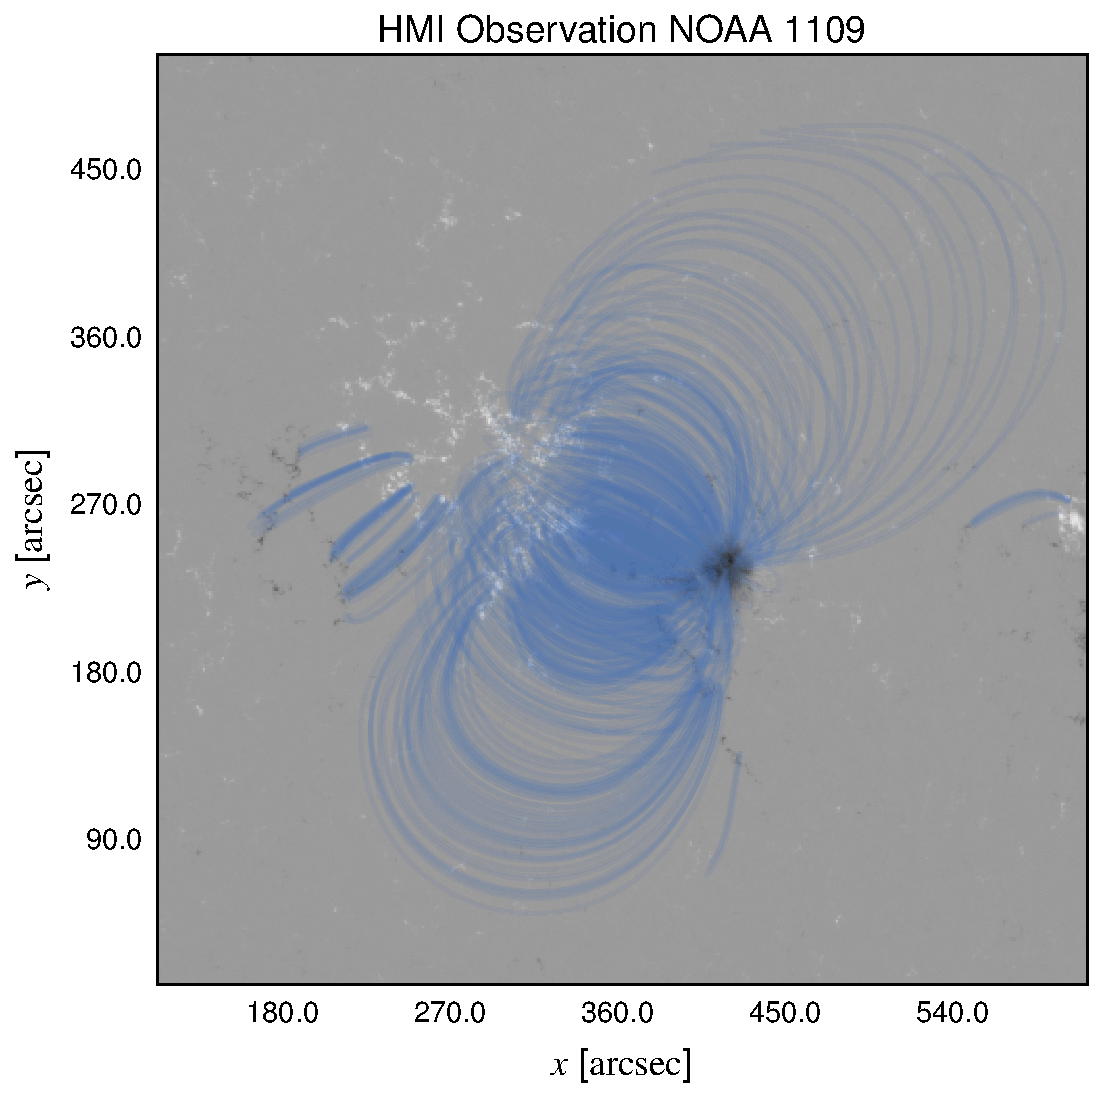
\includegraphics[width=\columnwidth]{figures/hmi_map_with_lines.pdf}
          \caption{Magnetogram of AR NOAA 1109 as observed by HMI on 29 September 2010 23:51:45 UTC. The 1000 fieldlines traced through the resulting potential field extrapolation are overplotted in blue.}
        \label{fig:hmi_map_with_lines}
        \end{figure}
      \end{column}
      \end{columns}
    \end{block}
    %
    % Heating model
    %% Show tN distributions
    \begin{block}{Heating Model: Nanoflare Trains with Varying Frequency}
      \begin{columns}[T]
      \begin{column}{0.49\columnwidth}
        \begin{itemize}
        \item Nanoflare model of \citet{parker_nanoflares_1988}: corona heated by impulsive ($\ll\tau_{cool}$), low-energy ($\sim10^{24}$ erg) events produced by twisting, braiding of field lines rooted in the photosphere
        \item Each strand heated independently by repeating triangular pulses of duration $\tau=200$ s; preferentially heat electrons 
        \item Use extrapolated field strength to estimate total energy input per strand as,
          \begin{equation*}
            E = (\epsilon B)^2/8\pi
          \end{equation*}
        \item $\epsilon=0.1$ is the stressing coefficient and $B$ is the average field strength per strand
        \item Event energies chosen from a power-law distribution with $\alpha=-2.5$ such that total energy constrained by above equation
        \item Choose four different average waiting times $\langle t_N\rangle=250,\,750,\,2500,\,5000$ s 
        \begin{itemize}
          \item Range from high-frequency heating (250 s) to low-frequency heating (5000 s)
          \item $t_{N,i}\propto E_i$ such that larger events require a longer ``winding time'', consistent with Parker nanoflare picture \citep[e.g.][]{cargill_active_2014,barnes_inference_2016-1}
        \end{itemize}
        \end{itemize}
      \end{column}
      \begin{column}{0.49\columnwidth}
        \begin{figure}
        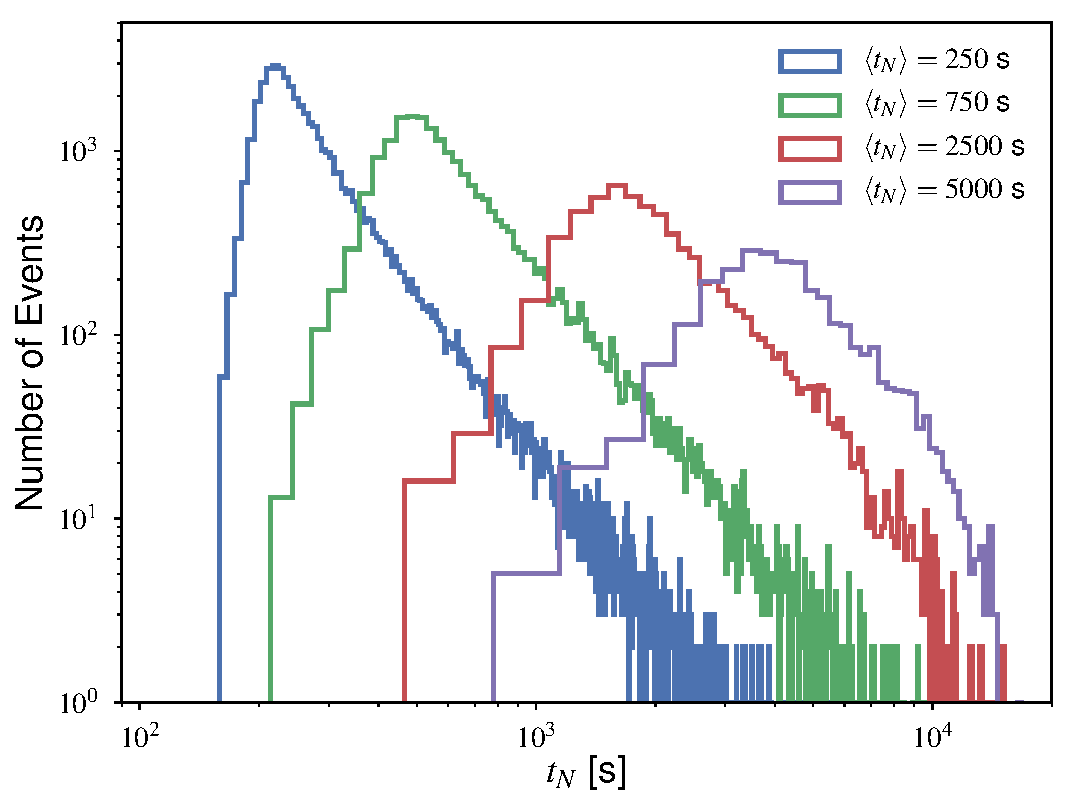
\includegraphics[width=\columnwidth]{figures/wait_time_distributions.pdf}
        \caption{Distribution of wait times $t_N$ for four average heating frequencies. Note that the total simulation time is fixed so there are more events in the high-frequency cases than in the low-frequency cases} 
        \label{fig:wait_times}
        \end{figure}
      \end{column}
      \end{columns}
    \end{block}
    %
    % Spectroscopic details/atomic physics
    %% What lines are we modeling? 
    \begin{block}{Spectroscopic Details}
      \begin{itemize}
        \item Calculate wavelelength-resolved intensity for 22 spectral lines studied by \citet{warren_systematic_2012} (see Table \ref{tab:line_table})
        \item Good coverage over the temperature range $0.5<T<6$ MK and inside passbands of \textit{Hinode}/EIS instrument
      \end{itemize}
      %
      \begin{columns}[T]
        \begin{column}{0.49\columnwidth}
          \begin{figure}
            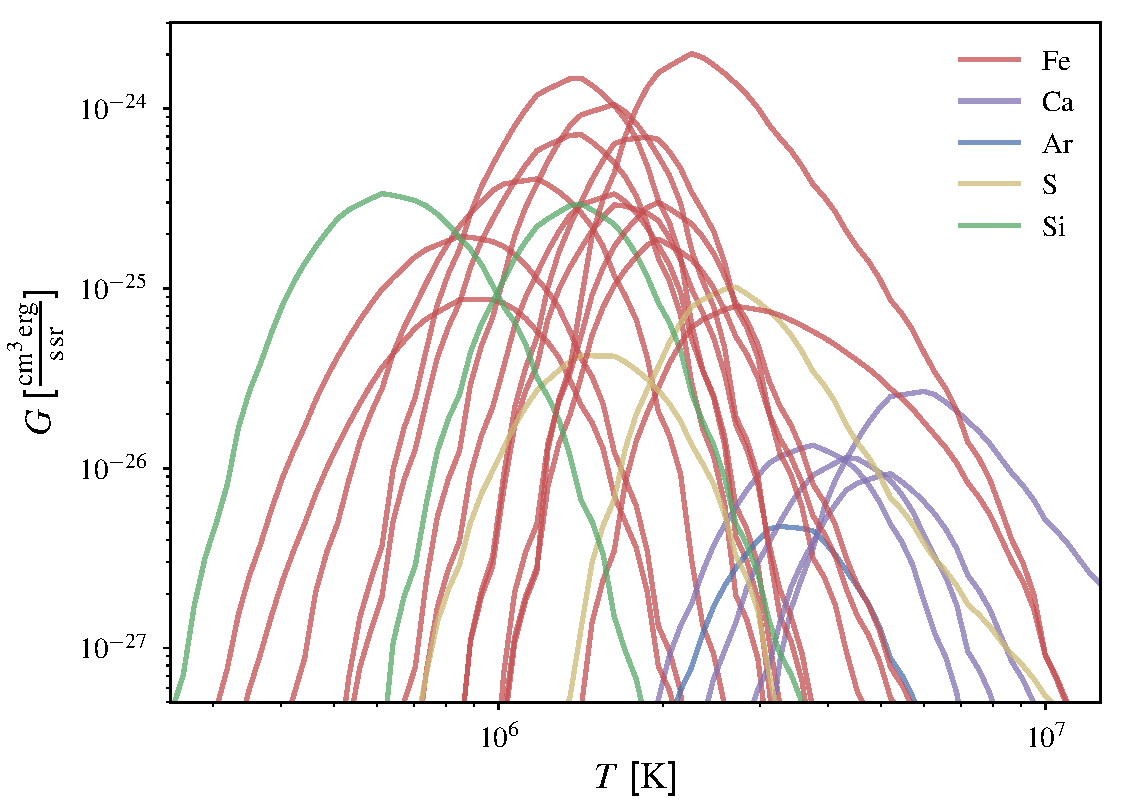
\includegraphics[width=\columnwidth]{figures/contribution_functions.pdf}
            \caption{Contribution functions for the 22 lines included in our model calculated assuming ionization equilibrium and a constant pressure of $p=10^{15}$ K/$\mathrm{cm}^{-3}$.}    
          \end{figure}
        \end{column}
        \begin{column}{0.49\columnwidth}
          \vspace{2ex}
          \begin{table}
            \centering
            \begin{minipage}{0.49\columnwidth}
              \begin{tabular}{|c|c|}
\hline
Ion & Wavelength [$\mathrm{\mathring{A}}$] \\
\hline\hline
Fe XI & 180.401 \\
Fe X & 184.537 \\
Fe XI & 188.216 \\
Fe IX & 188.493 \\
Fe XII & 192.394 \\
Ca XVII & 192.853 \\
Ca XIV & 193.866 \\
Ar XIV & 194.401 \\
Fe XII & 195.119 \\
Fe IX & 197.854 \\
Ca XV & 200.972 \\
\hline
\end{tabular}

            \end{minipage}
            \begin{minipage}{0.49\columnwidth}
              \begin{tabular}{|c|c|}
\hline
Ion & Wavelength [$\mathrm{\mathring{A}}$] \\
\hline\hline
Fe XIII & 202.044 \\
Fe XIII & 203.826 \\
Ca XVI & 208.585 \\
S XIII & 256.685 \\
Si X & 258.374 \\
Fe XVI & 262.976 \\
S X & 264.231 \\
Fe XIV & 264.789 \\
Fe XIV & 270.521 \\
Si VII & 275.361 \\
Fe XV & 284.163 \\
\hline
\end{tabular}

            \end{minipage}
            \caption{Selected wavelength-resolved transitions. All relevant atomic data are obtained from the CHIANTI database. These are the same lines chosen by \citet{warren_systematic_2012} to study NOAA 1109. \label{tab:line_table}}
          \end{table}
        \end{column}
      \end{columns}
    \end{block}
    %
    % EM diagnostics
    %% how to calculate true versus predicted EM
    \begin{block}{Emission Measure Diagnostics}
      \begin{itemize}
        \item \textit{True} emission measure from simulated thermodynamic quantities,
              \begin{equation*}
                \mathrm{EM}(T) = \int_{\mathrm{LOS}}\mathrm{d}h\,n^2(h,T)
              \end{equation*} 
        \item Bin in temperature $5.6<\log{T}<7.0$ with width $\Delta\log{T}=0.05$
        \item \textit{Predicted} EM from regularized inversion code of \citet{hannah_differential_2012}
        \item Assume 25\% uncertainty on our intensities to balance acceptable $\chi^2$ and smoothness
        \item Emission measure slope $\mathrm{EM}\sim T^a,\,\,6.0<\log{T}<\log{T_{peak}}$ often used as a diagnostic for heating frequency
        \item Fit power-law to cool side such that $\mathrm{EM}\sim T^a$
        \begin{itemize}
          \item Fit between 1 MK and $T_{peak}$ (4 MK true, 3 MK predicted), where $\mathrm{EM}_{max}=\mathrm{EM}(T_{peak})$
          \item Only fit to pixels where $\mathrm{EM}(T)>10^{25}\,\,\mathrm{cm}^{-5}$ and acceptable fit $R^2>0.9$
        \end{itemize}
      \end{itemize}
    \end{block}
  \end{column}
  %%
%%%%%%%%%%%%%%%%%%%%%%%%%%%%%%%%%%%%%%%%%%%%%%%%%
  %%second column
  \begin{column}{0.49\linewidth}
    %
    % em distributions
    %% maps of true versus predicted EM for a all tN and a few T bins
    \begin{block}{Total Emission Measure Maps}
      \begin{figure}
        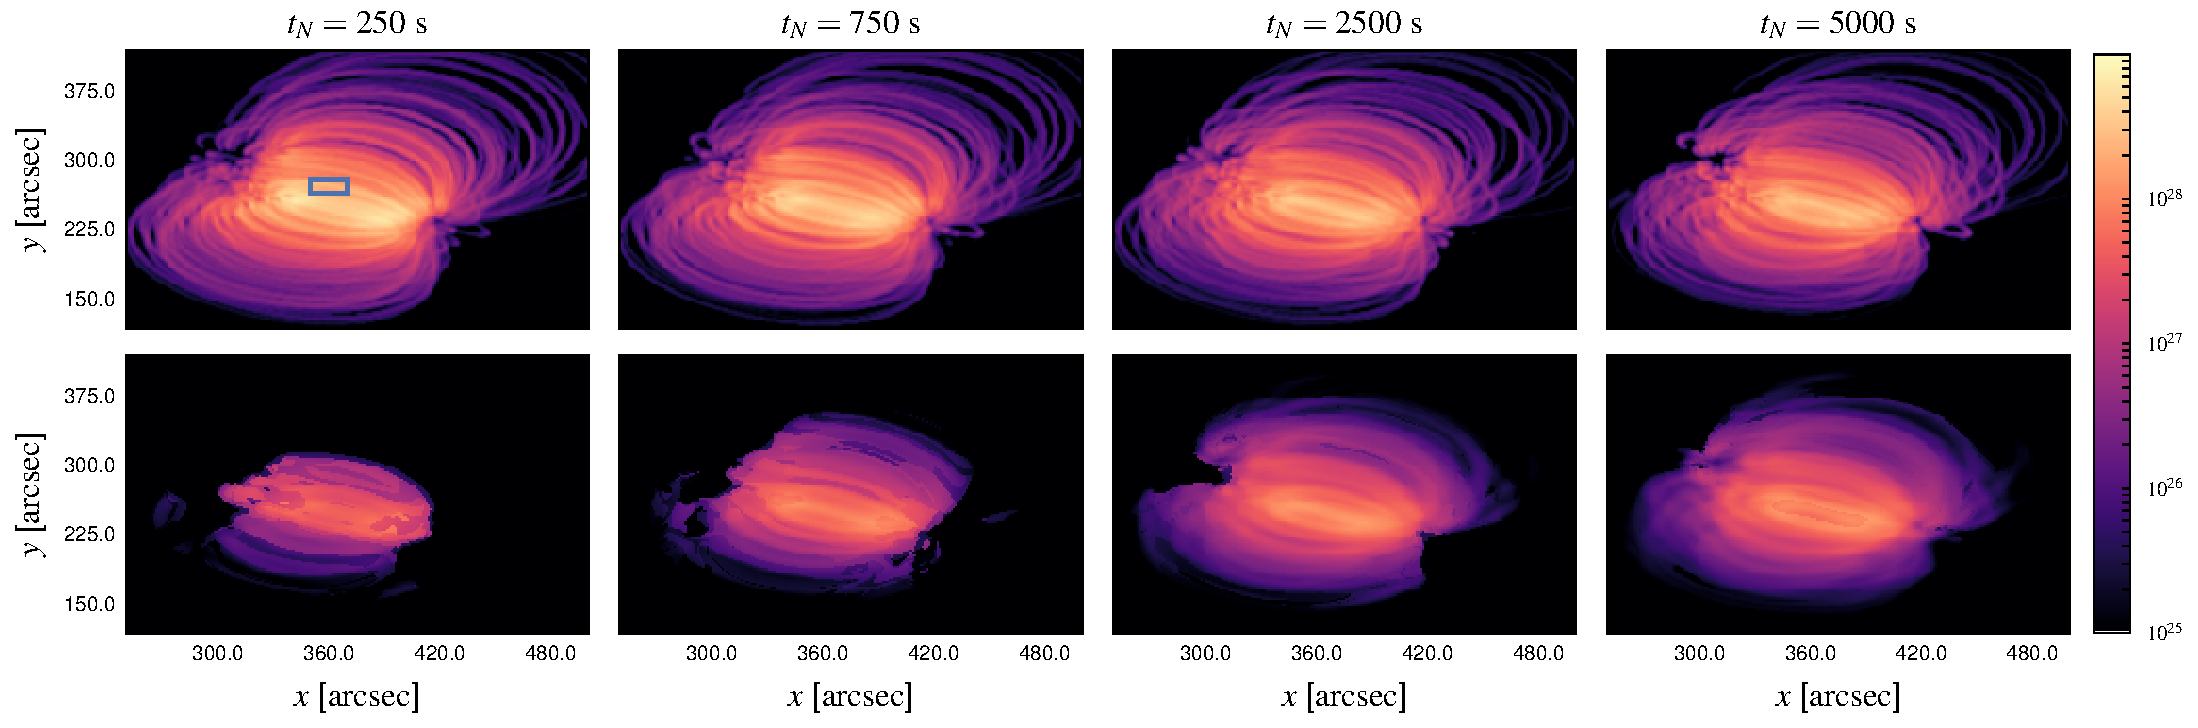
\includegraphics[width=\columnwidth]{figures/total_em_maps.pdf}
        \caption{Emission measure summed over all temperature bins for the true (top row) and predicted (bottom row) $\mathrm{EM}(T)$ for all four heating frequencies. The blue square in the top leftmost panel indicates the the area over which the $\mathrm{EM}(T)$ in Fig. \ref{fig:em_1d} are calculated.} 
        \label{fig:total_em_map}
      \end{figure}
    \end{block}
    %
    % em slopes
    %% maps of em slopes
    \begin{block}{Comparing Emission Measure Distributions: True versus Predicted}
      \begin{figure}
        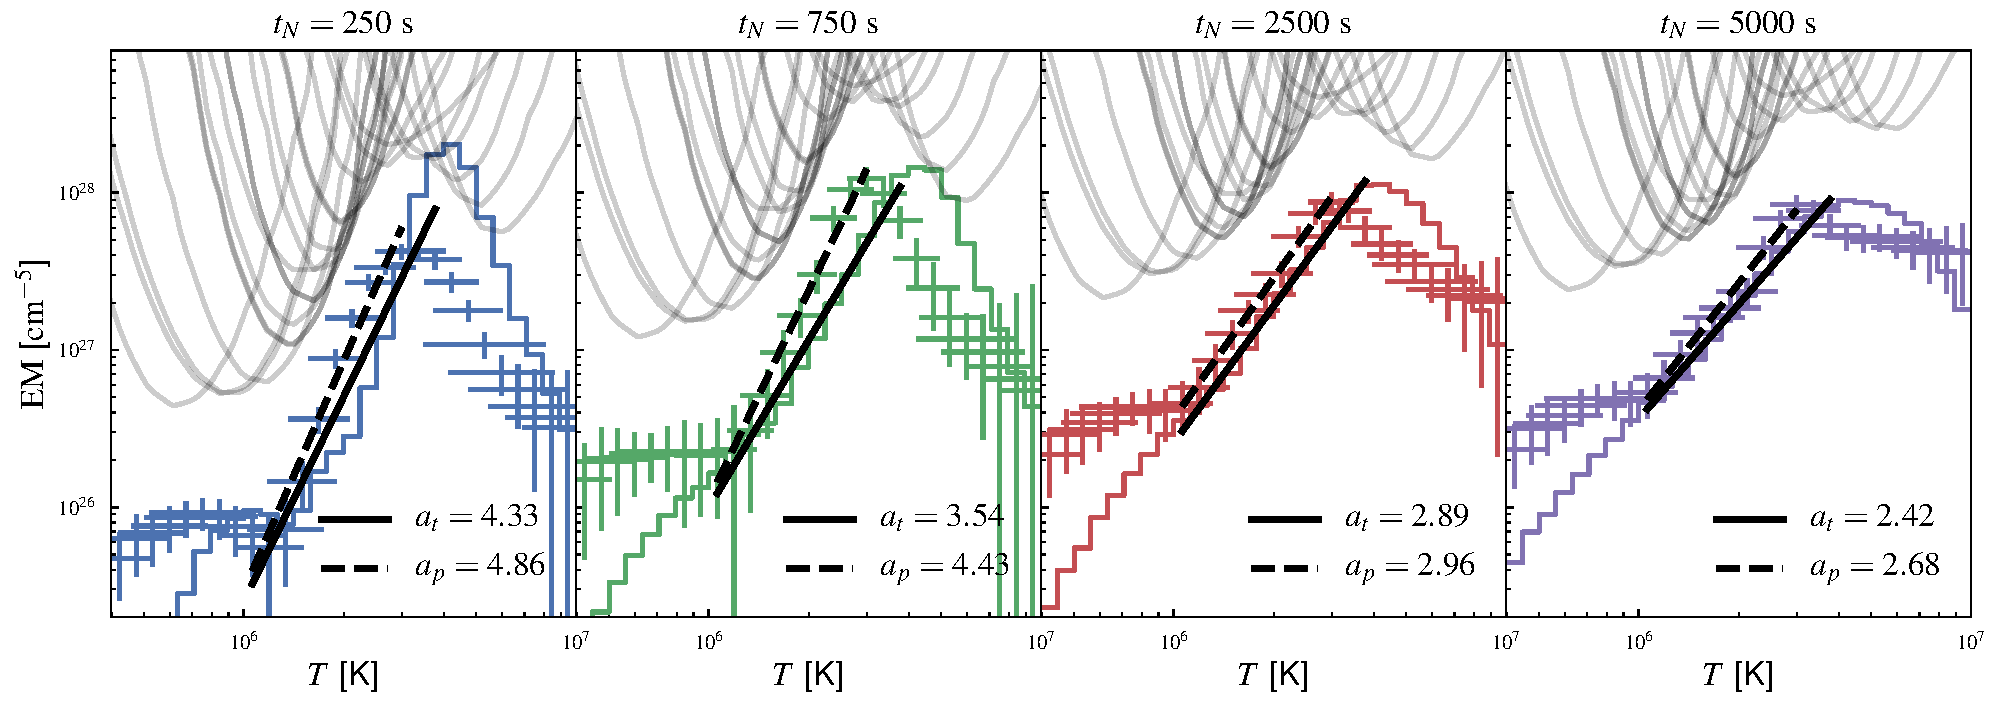
\includegraphics[width=\columnwidth]{figures/em_1d_compare.pdf}
        \caption{Pixel-averaged emission measure distributions calculated over the region indicated by the blue box in the top left panel of Fig. \ref{fig:total_em_map}. The true results are denoted by a solid line while the predicted results are denoted by errorbars in both the $T$ and $\mathrm{EM}$ direction. The EM-loci curves for all 22 spectral lines are shown in black. Additionally, a power-law has been fit between 1 MK and 4 MK (3 MK) for the true (predicted) case and is indicated by a solid (dashed) black line. Note that for all values of $t_N$, the predicted $\mathrm{EM}(T)$ peaks at lower temperatures as compared the true $\mathrm{EM}(T)$. The predicted $\mathrm{EM}(T)$ also tend to have steeper slopes, particularly in the higher-frequency cases.}
        \label{fig:em_1d}
      \end{figure}
    \end{block}
    %
    % em slopes
    %% maps of em slopes
    \begin{block}{Emission Measure Slope Maps}
      \begin{figure}
        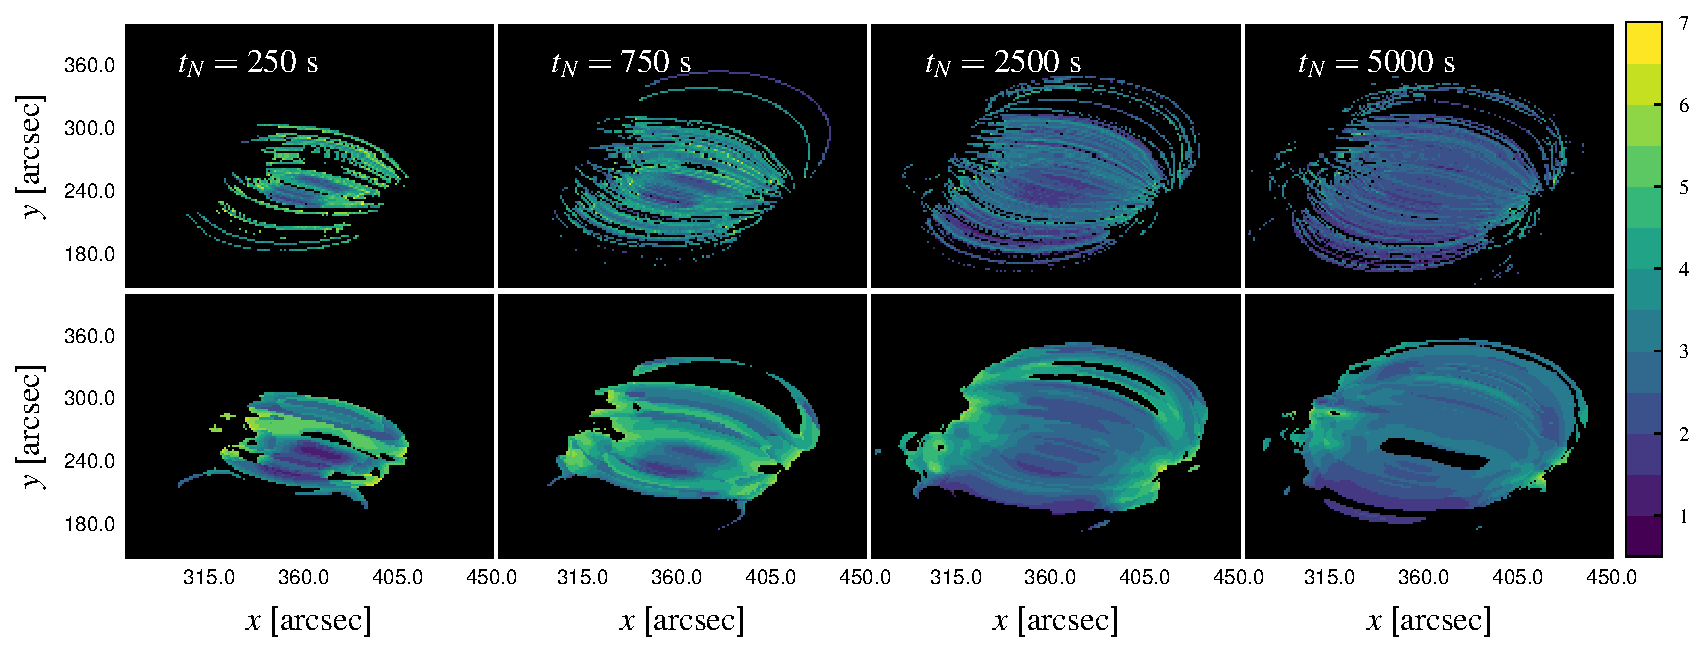
\includegraphics[width=\columnwidth]{figures/em_slope_maps.pdf}
        \caption{Maps of emission measure slopes, $a$, calculated from the true (top row) and predicted (bottom row) $\mathrm{EM}(T)$. The relative smoothness in the predicted $a$ values is due mostly to the ``fuzziness'' from the point spread function that is introduced when synthesizing the EIS intensities.}
        \label{fig:em_slope_maps}
      \end{figure}
    \end{block}
    %
    % em slope distributions
    %% distribution of slopes plus overplotted results from literature
    \begin{block}{Slope Distributions and Comparisons with Observations}
      \begin{figure}
        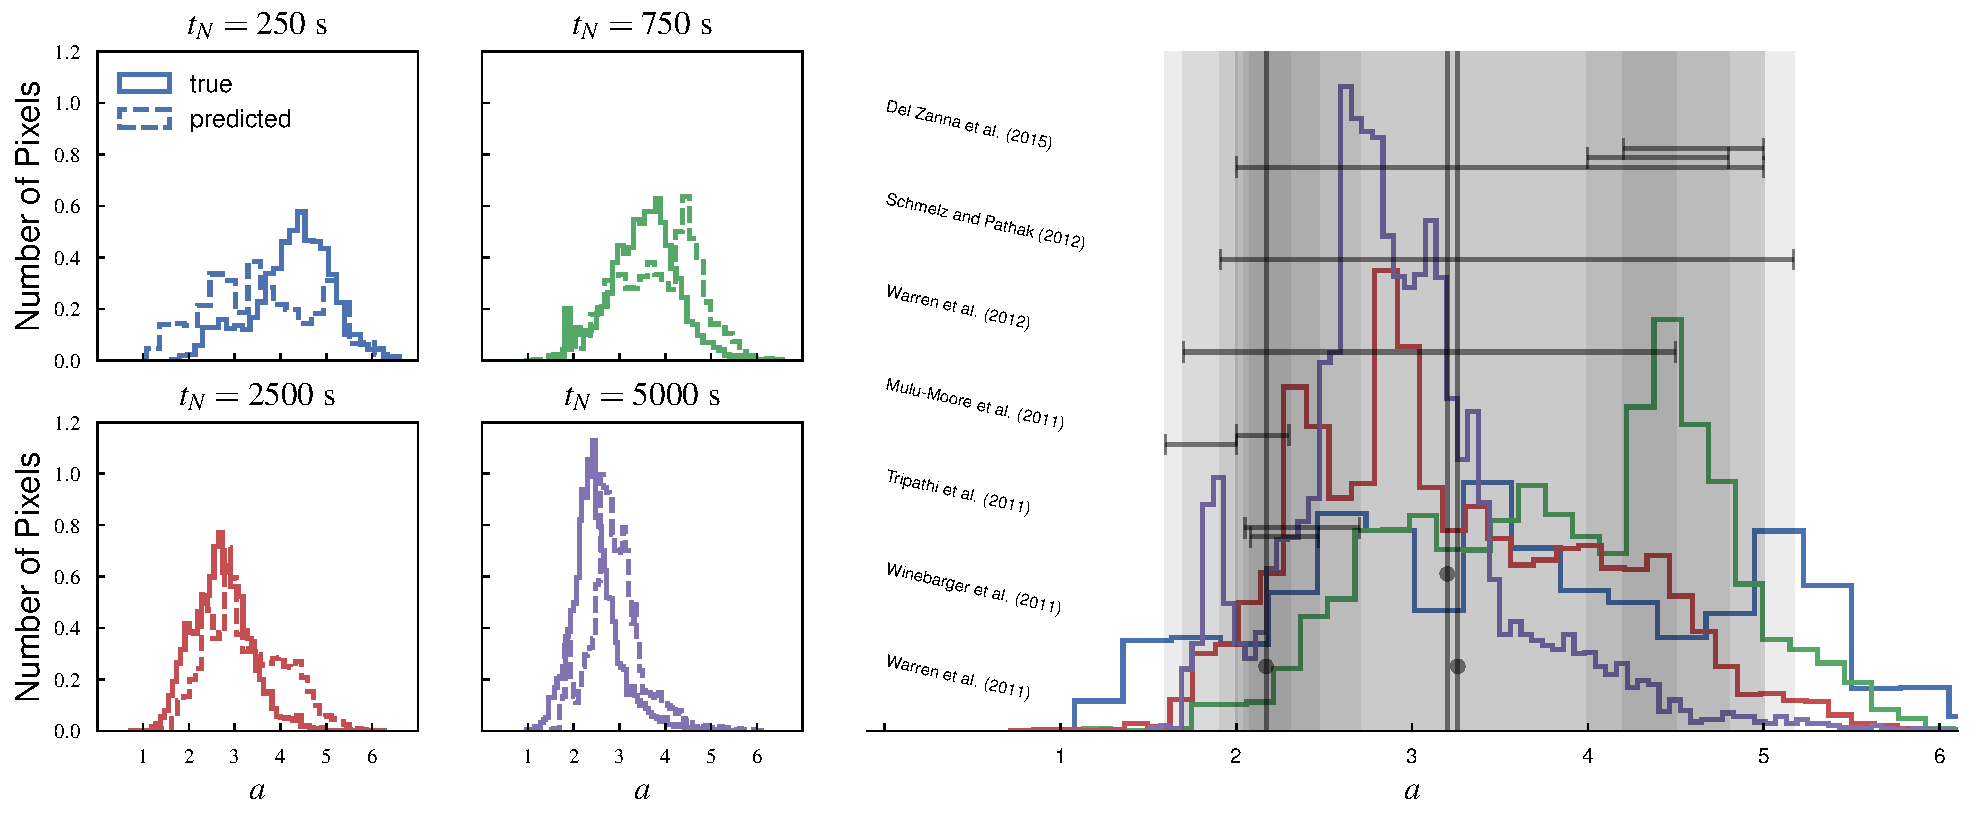
\includegraphics[width=\columnwidth]{figures/slope_distributions.pdf}
        \caption{\textbf{Left:} Normalized $\mathrm{EM}(T)$ slope distributions for every pixel in the synthesized AR. The slopes calculated from the true (predicted) $\mathrm{EM}(T)$ are denoted by a solid (dashed) line. Note that the $a$ distributions from the true $\mathrm{EM}(T)$ tend to be more sharply peaked and show a clearly inverse relation to $t_N$, consistent with other workers \citep[e.g.][]{cargill_active_2014}. \textbf{Right:} Normalized distributions of $a$ values from the predicted $\mathrm{EM}(T)$ overlaid on observed results from the literature. Studies that reported a range of $a$ values are indicated by a shaded block and an error bar while those studies that reported only a single value are denoted by a circle and vertical bar. Note that the spread of observed values is nearly as wide as all of our predicted $a$ distributions.}
        \label{fig:slope_dist}
      \end{figure}
    \end{block}
    %
    %Conclusions
    \begin{block}{Conclusions}
      \begin{itemize}
        \item Global active region modeling a powerful tool for studying dynamically-heated AR cores
        \item Relationship between predicted $a$ and $t_N$ \alert{much ``messier'' compared to true $\mathrm{EM}$}
        \item Predicted $\mathrm{EM}$ peak at lower temperatures than true $\mathrm{EM}$, independent of heating frequency
        \item Observed slopes most consistent with intermediate to low frequency heating, but spread is large
        \item \alert{Caution when computing emission measure from model results}
      \end{itemize}
    \end{block}
    %
    %references
    \begin{block}{References}
      \scriptsize
      \begin{multicols}{2}
        \bibliographystyle{apj}
        \bibliography{references.bib}
      \end{multicols}
    \end{block}
  \end{column}
  \end{columns}
\end{frame}
\end{document}
